\begin{frame}
\frametitle{Arquivo .tex}
\framesubtitle{principal arquivo do seu documento}
O arquivo .tex será o principal arquivo do seu documento. Neste arquivo você incluirá/definirá:
\begin{itemize}
    \item classe do documento
    \item tamanho de fonte, tamanho da página, coluna simples ou dupla, etc
    \item pacotes
    \item texto, figuras, tabelas, equações
    \item outros arquivos .tex
    \item bibliografia
\end{itemize}
\end{frame}


\begin{frame}[fragile]
\frametitle{Espaços em branco}
\framesubtitle{}
  Um ou vários espaços em branco são tratados como um único espaço em branco.
\begin{LTXexample}
Não interessa se introduz apenas
um ou vários     espaços depois
de uma palavra.

Uma linha em branco inicia um novo
parágrafo. 
\end{LTXexample}
\end{frame}


\begin{frame}[fragile]
\frametitle{Caracteres reservados}
\framesubtitle{}
Alguns caracteres são reservados:
\begin{verbatim}
#  $  %  ^  &  _  {  }  ~  \ 
\end{verbatim}

Para escrever um desses caracteres é necessário utilizar o caractere de escape.
  \vspace{1cm}
\begin{LTXexample}[commentstyle=\color{black}]
  \# \$ \% \^{} \& \_ \{ \} \~{} \textbackslash
\end{LTXexample}
\end{frame}


\begin{frame}[fragile]
\frametitle{Comandos}
\framesubtitle{}
Começam com um backslash e têm um nome que consiste apenas de letras. Os comandos obedecem à seguinte sintaxe:

\begin{verbatim}
\commandname[option1,option2,...]{argument1}{argument2}...
\end{verbatim}

\begin{LTXexample}
Li que o Knuth divide as
pessoas que trabalham com o \TeX{}
em \TeX{}nicos e \TeX pertos.\\
Hoje é \today.
\end{LTXexample}
\end{frame}


\begin{frame}[fragile]
\frametitle{Ambientes}
Os ambientes são utilizados para formatar blocos de texto em \LaTeX{}.
Os ambientes possuem a seguinte sintaxe:

\begin{verbatim}
\begin{environment_name}{arguments}[optional_arguments]
...
\end{environment_name}
\end{verbatim}

\begin{LTXexample}
\begin{center}
\lipsum[1][1-4]
\end{center}
\end{LTXexample}

\end{frame}


\begin{frame}[fragile]
\frametitle{Comentários}
\framesubtitle{}
Tudo o que vem após o carácter \% é um comentário. Podemos também fazer comentários em bloco.

\begin{LTXexample}
Este é um % estúpido
% Melhor: instrutivo <----
exemplo: Supercal%
ifragilist%
icexpialidocious

Este é outro
\begin{comment}
bastante estúpido,
mas instrutivo
\end{comment}
exemplo de como embeber
comentários nos seus documentos.
\end{LTXexample}:
\end{frame}

\begin{frame}[fragile]
\frametitle{Estrutura}
\framesubtitle{}
  A seguinte estrutura é esperada em um arquivo \LaTeX{}.

\begin{verbatim}
\documentclass{...}
\usepackage{...}
...
\begin{document}
...
\end{document}
\end{verbatim}
\end{frame}

\begin{frame}[fragile]
\frametitle{Exemplo}
\framesubtitle{}
  \scriptsize
  \begin{columns}[c]
  \column{.5\textwidth}
  \begin{figure}[h!]
  \centering
  \setlength\fboxsep{0pt}
  \setlength\fboxrule{0.5pt}
  \fbox{
\includegraphics[width=0.7\textwidth,height=0.8\textheight,keepaspectratio]{minimal.pdf}}
  \label{fig:minimal}
  \end{figure}
  \column{.5\textwidth}
  \begin{verbatim}
\documentclass{article}
% esta linha é específica para
% o Português e outras línguas
% com caracteres acentuados.
\usepackage[latin1]{inputenc}
\begin{document}
Pequeno é belo.
\end{document}
\end{verbatim}
  \end{columns}
\end{frame}

\begin{frame}[fragile]
\frametitle{Exemplo 2}
\framesubtitle{}
  \scriptsize
  \begin{columns}[c]
  \column{.5\textwidth}
  \begin{figure}[h!]
  \centering
  \setlength\fboxsep{0pt}
  \setlength\fboxrule{0.5pt}
  \fbox{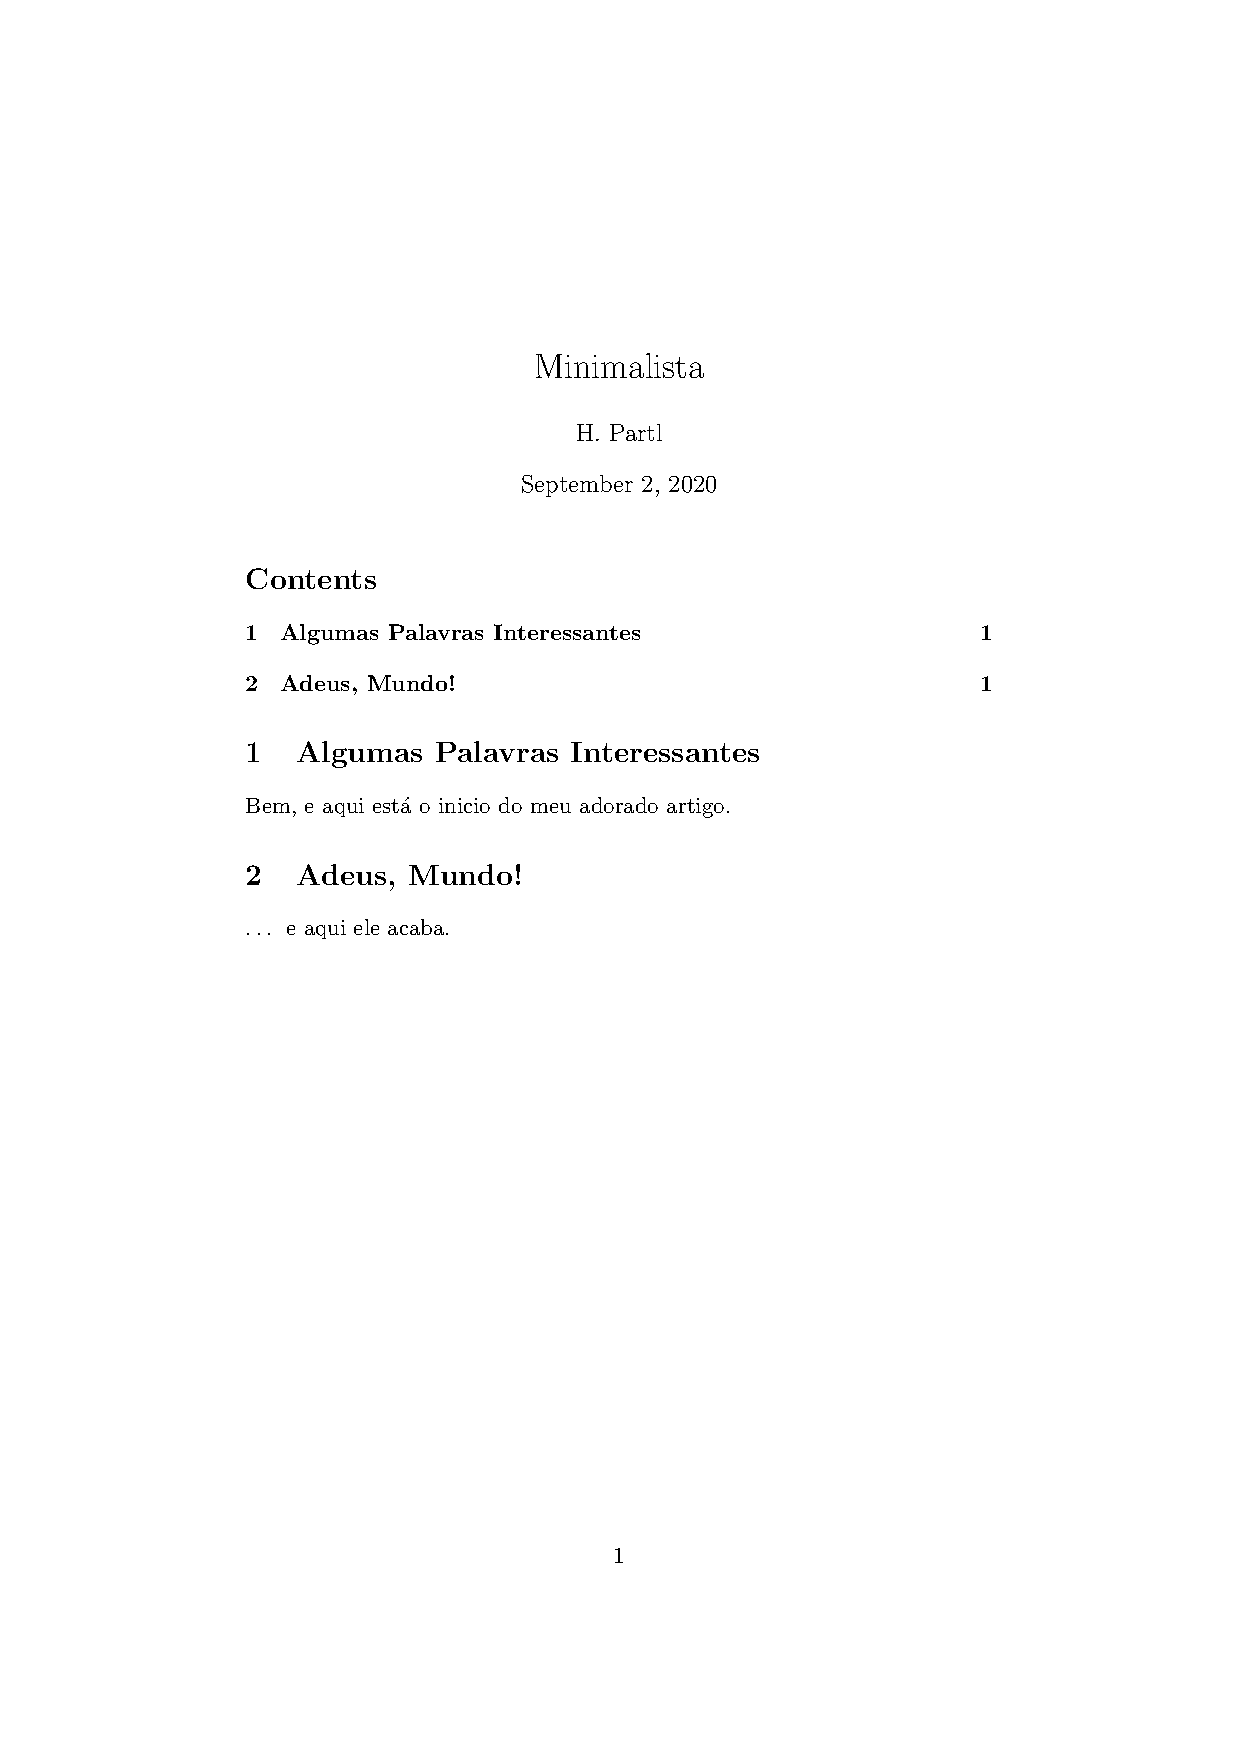
\includegraphics[width=0.7\textwidth,height=0.8\textheight,keepaspectratio]{minimal2.pdf}}
  \label{fig:minimal2}
  \end{figure}
  \column{.5\textwidth}
\begin{verbatim}
\documentclass[a4paper,11pt]{article}
% Esta linha é necessária para
% documentos em línguas que incluam
% caracteres acentuados.
\usepackage[latin1]{inputenc}
% Define o autor e título
\author{H.Partl}
\title{Minimalista}
\begin{document}
% Gera o título
\maketitle
% Insere a tabela de conteúdos
\tableofcontents
\section{Algumas Palavras Interessantes}
Bem, e aqui está o inicio do meu adorado artigo.
\section{Adeus, Mundo!}
\ldots{} e aqui ele acaba.
\end{document}
\end{verbatim}
  \end{columns}
\end{frame}


\subsection{Classes}
\begin{frame}[fragile,allowframebreaks]
\frametitle{Documento}
\framesubtitle{classes de documento}
  \begin{verbatim}
  \documentclass[opções]{classe}
  \end{verbatim}
  Exemplo:
  \begin{verbatim}
  \documentclass[11pt,twoside,a4paper]{article}
  \end{verbatim}

  Classes
  \begin{description}
  \item[article] para artigos em jornais científicos, pequenos relatórios, documentação de programas, convites, ...
  \item[report] para relatórios mais longos contendo vários capítulos, pequenos livros, teses de doutorado, ...  
  \item[book] para livros
  \item[slides] para slides. Esta classe usa letras grandes do tipo sans serif. Deve-se
       considerar utilizar o pacote Beamer.
  \end{description}

  \framebreak
  Pacotes de classes:
  \begin{itemize}
  \item \hrefcolor{https://ctan.org/pkg/koma-script}{KOMA-Script} fornece as seguintes classes: \emph{article}, \emph{report}, \emph{book} e \emph{letter}.
    As classes do KOMA-Script seguem o estilo dado pelo tipógrafo Jan Tschichold.
  \item \hrefcolor{https://www.ctan.org/pkg/memoir}{memoir} fornece classes para poesias, trabalhos matemáticos, obras ficcionais e não ficcionais.
  \item \hrefcolor{https://ctan.org/pkg/beamer}{beamer} é uma classe para apresentações em slides.
  \item \hrefcolor{https://ctan.org/pkg/sciposter}{sciposter} é uma classe para posters científicos.
  \end{itemize}

\end{frame}

\begin{frame}
\frametitle{Classes}
\framesubtitle{atributos das classes}
  Opções:

  \begin{description}[a4paper, b5paper, letterpaper]
  \item[10pt, 11pt, 12pt] para definir o tamanho da fonte
  \item[a4paper, b5paper, letterpaper] para definir o tamanho do papel
  \item[titlepage, notitlepage] especifica se se deve criar uma nova página depois do título do documento ou não
  \item[twocolumn, onecolumn] documento em duas colunas
  \item[twoside, oneside] impressão frente-verso ou não  
  \item[openright, openany] faz os capítulos começarem apenas nas páginas do lado direito ou na próxima disponível
  \item[landscape] formato paisagem
  \item[outras] depende de cada classe
  \end{description}
\end{frame}



\begin{frame}[label={clsfile}]
\frametitle{Arquivo de classe de documento, arquivo de estilo e pacote}
\framesubtitle{.cls e .sty}
Qualquer um pode definir sua própria classe.

\vspace{6ex}
Veja o tutorial no  \hrefcolor{https://www.overleaf.com/learn/latex/Understanding_packages_and_class_files}{Overleaf}
\end{frame}



\subsection{Documento .tex}
\begin{frame}[fragile]
\frametitle{Documento}
\framesubtitle{Incluir um documento em outro documento}
  Pomos incluir um arquivo \texttt{.tex} dentro de outro. Para tanto, basta fazer:
  
  \begin{verbatim}
  \input{nome_do_arquivo}
  
  \include{nome_do_arquivo} 
  equivalente a 
  \clearpage \input{nome_do_arquivo} \clearpage
  \end{verbatim}
\end{frame}



\begin{frame}[fragile]
\frametitle{Documento}
\framesubtitle{Comandos de Secção}
  
\begin{verbatim}
\part{}

\chapter{}

\section{}

\subsection{}

\subsubsection{}

\paragraph{}
\end{verbatim}

\end{frame}



\begin{frame}[fragile]
\frametitle{Documento}
\framesubtitle{quebra de linha e nova página}
\begin{LTXexample}
  você pode \\ quebrar uma linha 
  quando quiser no \newline \LaTeX, 
  entretanto uma simples quebra
  de linha do código não reflete 
  em quebra de linha... 
  
  mas você pode deixar uma linha 
  em branco
\end{LTXexample}  
  Comando utilizado para iniciar uma nova página: \verb|\newpage|
\end{frame}


\begin{frame}[fragile]
\frametitle{Documento}
\framesubtitle{Hifenização de palavras}
  \begin{verbatim}
\hyphenation{lista de palavras}
  \end{verbatim}

\begin{LTXexample}
  \hyphenation{MINICURSOLATEX uni-ver-si-da-de}
  Penso que isto é: su\-per\-cal\-%
  i\-frag\-i\-lis\-tic\-ex\-pi\-%
  al\-i\-do\-cious
  
  Teste de hifenização da palavra 
  universidade, inclusive de  
  certa  palavra MINICURSOLATEX, 
  que não deve ser hifenizada.
\end{LTXexample}
\end{frame}


\begin{frame}[fragile]
\frametitle{Documento}
\framesubtitle{Estilo de fonte em um texto}
\begin{LTXexample}
  \textbf{Bold} \\
  \textit{Italic} \\
  \texttt{Monotype} \\
  \textsf{Sans Serif} \\
  \textsc{SmallCaps} \\
  \textsl{Slanted} \\
  \emph{Enfase}
\end{LTXexample}
\end{frame}


\begin{frame}[fragile]
\frametitle{Documento}
\framesubtitle{Tamanho da fonte em um texto}
\begin{LTXexample}
  {\tiny texto texto ...} \\
  {\scriptsize texto texto ...} \\
  {\footnotesize texto texto ...} \\
  {\small texto texto ...} \\
  {\normalsize texto texto ...} \\
  {\large texto texto ...} \\
  {\Large texto texto ...} \\
  {\LARGE texto texto ...} \\
  {\huge texto texto ...} \\
  {\Huge texto texto ...}
\end{LTXexample}
\end{frame}

\begin{frame}[fragile]
\frametitle{Documento}
\framesubtitle{Alinhamento de texto}
\begin{LTXexample}
  \begin{center}
  texto texto
  \end{center}
  \begin{flushleft}
  texto texto
  \end{flushleft}
  \begin{flushright}
  texto texto
  \end{flushright}
\end{LTXexample}
\end{frame}

\begin{frame}[fragile]
\frametitle{Documento}
\framesubtitle{Layout de uma página}
  \scriptsize
  \begin{columns}[c]
  \column{.5\textwidth}
  \begin{itemize}
  \item \verb|\hoffset|
  \item \verb|\voffset|
  \item \verb|\oddsidemargin|
  \item \verb|\topmargin|
  \item \verb|\headheight|
  \item \verb|\headsep|
  \item \verb|\textheight| 
  \item \verb|\textwidth|
  \item \verb|\marginparsep|
  \item \verb|\marginparwidth|
  \item \verb|\footskip|
  \end{itemize}
  \column{.5\textwidth}
  \vspace{-1.5cm}
\begin{figure}[h!]
  \centering
  \label{fig:Latex_layout}
    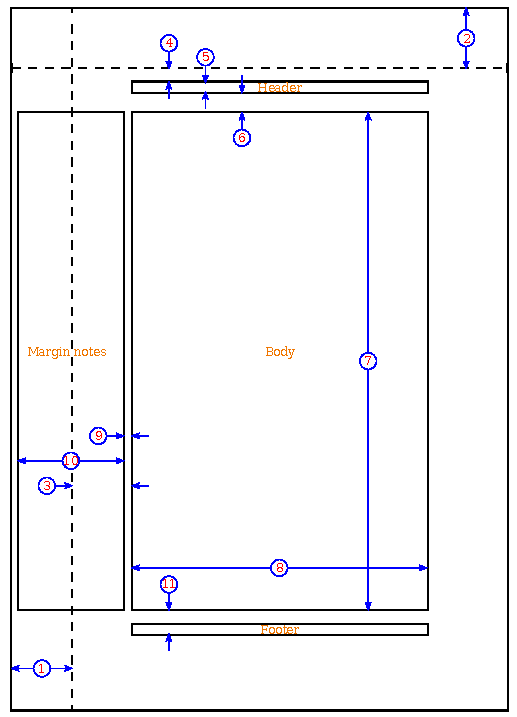
\includegraphics[width=0.8\textwidth,height=.95\textheight,keepaspectratio]{figures/Latex_layout.pdf}
  %\caption{Tux.}
\end{figure}
  \end{columns}
\end{frame}


\begin{frame}[fragile]
\frametitle{Documento}
\framesubtitle{Layout}
  \begin{verbatim}
\documentclass[a4paper]{article}
\usepackage[top=tlength, bottom=blength, left=llength,
        right=rlength]{geometry}
\usepackage[a4paper,landscape]{geometry}
  \end{verbatim} 
\end{frame}


\begin{frame}[fragile]
\frametitle{Documento}
\framesubtitle{Cabeçalho e Rodapé}
  \begin{verbatim}
\usepackage{fancyhdr}

\fancyhead[CE]{Author's Name}
\fancyhead[CO]{\today}
\fancyfoot[LE,RO]{\thepage}
  \end{verbatim} 
  
  \url{https://ctan.org/pkg/fancyhdr} \\
  \url{https://www.overleaf.com/learn/latex/Headers_and_footers}
\end{frame}


\begin{frame}[fragile]
\frametitle{Documento}
\framesubtitle{misturar coluna simples com multiplas colunas}

\small
\begin{LTXexample}
\lipsum[1][1-2]
\begin{multicols}{2}
\lipsum[1][3-6]
\end{multicols}
\lipsum[1][7-9]
\end{LTXexample}

\url{https://www.ctan.org/pkg/multicol} \\
\url{https://www.overleaf.com/learn/latex/Multiple_columns}
\end{frame}


\begin{frame}[fragile]
\frametitle{Documento}
\framesubtitle{Notas de rodapé}
\begin{LTXexample}
No meio do texto, podemos colocar a nota de rodapé\footnote{Nota que fica na
parte inferior da página.} para explicações adicionais tais como significado da
palavra, ou fonte que foi usada.
\end{LTXexample}
No meio do texto, podemos colocar a nota de rodapé\footnote{Nota que fica na
parte inferior da página.} para explicações adicionais tais como significado da
palavra, ou fonte que foi usada.
\end{frame}

\begin{frame}[fragile]
\frametitle{Documento}
\framesubtitle{Sumário}
\begin{LTXexample}
\tableofcontents
\end{LTXexample}
\end{frame}


\begin{frame}[fragile]
\frametitle{Documento}
\framesubtitle{Sumário - local corrente}
\begin{LTXexample}
\tableofcontents[current,currentsection]
\end{LTXexample}
\end{frame}


%\subsection{Linguística}\label{sec:linguistica}
%\section{Linguística}

\begin{frame}[fragile]
\frametitle{Linguística}
\framesubtitle{Ferramentas para trabalhos em linguística}

\begin{enumerate}
    \item caracteres IPA
    \item árvores sintáticas
    \item árvores de dependências
    \item exemplos enumerados
\end{enumerate}

\end{frame}


\begin{frame}[fragile]
\frametitle{Linguística}
\framesubtitle{escrita fonética}
  \scriptsize
  \begin{columns}[c]
  \column{.5\textwidth}
  \begin{verbatim}
   \usepackage{tipa}
   
   \textipa{abcdefghijklmnopqrstuvwxyz}
   \textipa{ABCDEFGHIJKLMNOPQRSTUVWXYZ}
   \textipa{1234567890 @}
   \textipa{\:d \:l \:n \:r \:s \:t \:z}
   \textipa{\!b \!d \!g \!j \!G \!o}
  \end{verbatim}
  \column{.5\textwidth}
  \begin{fmpage}{\textwidth}
   \textipa{abcdefghijklmnopqrstuvwxyz}
   \textipa{ABCDEFGHIJKLMNOPQRSTUVWXYZ}
   \textipa{1234567890 @}
   \textipa{\:d \:l \:n \:r \:s \:t \:z}
   \textipa{\!b \!d \!g \!j \!G \!o}
  \end{fmpage}
  \end{columns}

  \url{https://www.tug.org/TUGboat/tb17-2/tb51rei.pdf}
  \url{https://ctan.org/pkg/tipa}

\end{frame}


\begin{frame}[fragile]
\frametitle{Linguística}
\framesubtitle{Tabela com códigos dos símbolos do IPA}
\vspace{-4ex}
\begin{figure}[h!]
  \centering
  \label{fig:tipachart}
  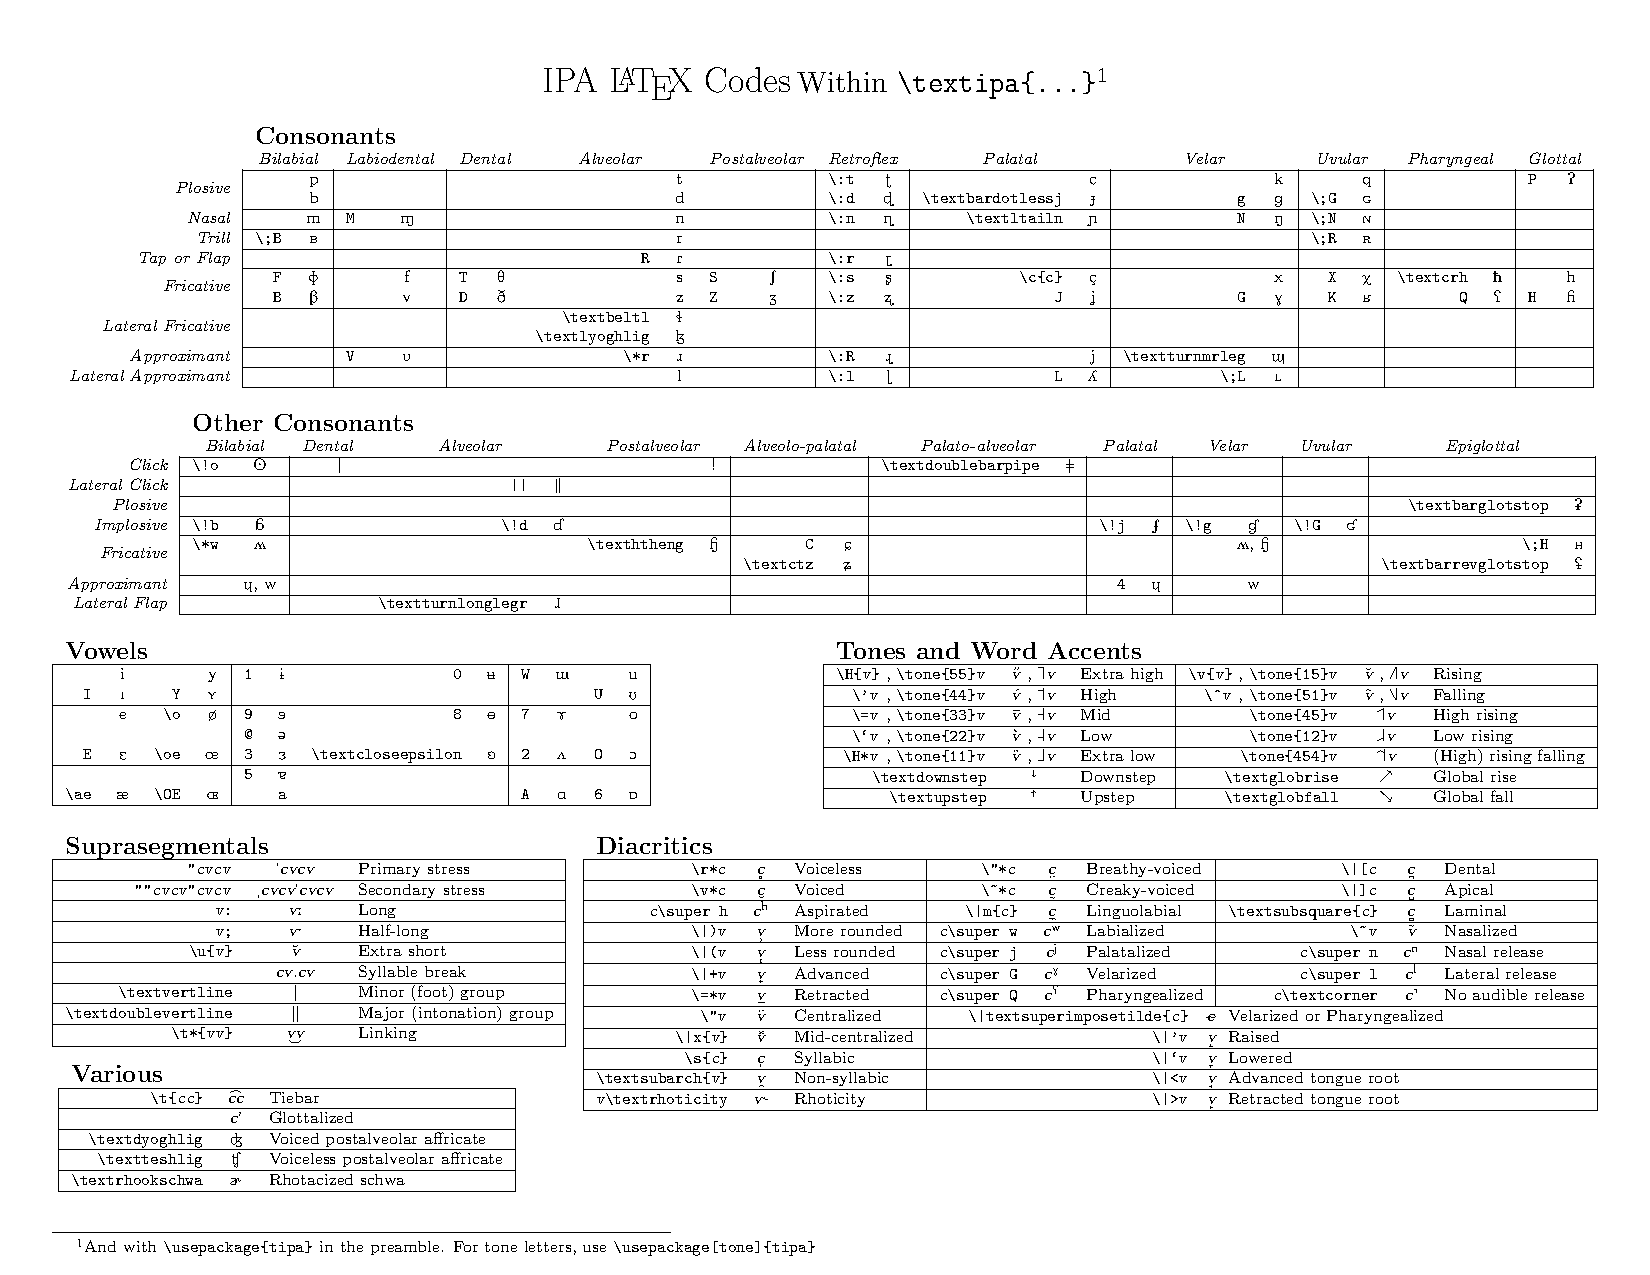
\includegraphics[width=0.7\textwidth,height=0.9\textheight,keepaspectratio]
                     {figures/tipachart_mod.pdf}
  %\caption{Tabela IPA.}
\end{figure}
\end{frame}


\begin{frame}[fragile]
\frametitle{Linguística}
\framesubtitle{Regras fonológicas}
  \scriptsize
  \begin{verbatim}
\usepackage{phonrule}
  
\phonb{\phonfeat{+stop \\ +consonant \\ +alveolar} }{[\textipa{R}]}
{\phonfeat{+vowel \\ +stressed} }{\phonfeat{+vowel \\ +stressed} }
  \end{verbatim}

  \begin{fmpage}{\textwidth}
\phonb{\phonfeat{+stop \\ +consonant \\ +alveolar} }{[\textipa{R}]}{\phonfeat{+vowel \\ +stressed} }{\phonfeat{+vowel \\ +stressed} }
  \end{fmpage}

\end{frame}


\begin{frame}[fragile]
\frametitle{Linguística}
\framesubtitle{Árvores sintáticas}
  \scriptsize
  \begin{columns}[c]
  \column{.5\textwidth}
  \begin{verbatim}
\usepackage{qtree}

\begin{center}
\Tree [.S [.NP LaTeX ] [.VP [.V is ] 
  [.NP fun ] ] ]
\end{center}
  \end{verbatim}
  \column{.5\textwidth}
  \begin{fmpage}{\textwidth}
\begin{center}
\Tree [.S [.NP LaTeX ] [.VP [.V is ] [.NP fun ] ] ]
\end{center}
  \end{fmpage}
  \end{columns}
\end{frame}

\begin{frame}[fragile]
\frametitle{Linguística}
\framesubtitle{Árvore de dependência}

  \begin{fmpage}{\textwidth}
   \begin{dependency}[theme = simple]
   \begin{deptext}[column sep=1em]
      A \& hearing \& is \& scheduled \& on \& the \& issue \& today \& . \\
   \end{deptext}
   \deproot{3}{ROOT}
   \depedge{2}{1}{ATT}
   \depedge[edge start x offset=-6pt]{2}{5}{ATT}
   \depedge{3}{2}{SBJ}
   \depedge{3}{9}{PU}
   \depedge{3}{4}{VC}
   \depedge{4}{8}{TMP}
   \depedge{5}{7}{PC}
   \depedge[arc angle=50]{7}{6}{ATT}
   \end{dependency}
  \end{fmpage}

\end{frame}



%\subsection{Notas e Citações}\label{sec:notascita}
%\input{notas.tex}

%\subsection{Comandos}\label{sec:comandos}
%\subsection{Comandos}

\begin{frame}[fragile,allowframebreaks]
\frametitle{Comandos}
Kunth definiu 325 primitivas para o \TeX{}.

\vspace{3ex}
O outros motores utilizam mais primitivas.
Veja: \hrefcolor{https://www.overleaf.com/learn/latex/TeX_primitives_listed_by_TeX_engine}{\TeX{} primitives listed by \TeX{ engine}}.


\vspace{3ex}
Outros comandos são definidos como combinações de primitivas ou de outros comandos.

\framebreak 

A formatação com \LaTeX{} é facilitada com a utilização de comandos.
Exemplos de comandos: \verb|\textbf{...}|, \verb|\url{...}|, \verb|\item|, etc.

\vspace{3ex}
Novos commandos podem ser definidos:
\begin{lstlisting}[language=tex, label=lst-comand-def, postbreak=\mbox{$\hookrightarrow$\space}, basicstyle=\fontsize{8}{10}\selectfont\ttfamily]
% comando simples (incluir \usepackage{amsfonts})
\newcommand{\R}{$\mathbb{R}$}

% comando com parametro
\newcommand{\bb}[1]{$\mathbb{#1}$} 

% (incluir \usepackage{hyperref})
\newcommand{\email}[1]{\href{mailto:#1}{#1}}
\end{lstlisting}

\framebreak

Comando com parâmetro opcional:
\begin{LTXexample}
\newcommand{\plusbinomial}[3][2]{(#2 + #3)^#1}

\[ \plusbinomial{x}{y} \]

\[ \plusbinomial[4]{y}{y} \]
\end{LTXexample}
\end{frame}





%\subsection{Bibliografia}\label{sec:bibtex}
%\input{bibliografia.tex}
